\subsection{Distributed Memory Model}
\sciwms{} decomposes an externally hosted dataset into a structure
(topology), defined as a geo-referenced spatial set of sample
locations and connections, with associated attributes.

\begin{figure}[ht!]
  \centering
  \includegraphics[width=\textwidth]{../figs/topology_memModel}
  \caption{\sciwms{} distributed memory model.}
  \label{fig:sciwms_mem_model}
\end{figure}

Fufilling a \wms{} request requires computing visible regions of a
topology, fetching attributes and using connectivity information to
produce an accurate rendering. The most computationally expensive
operation in this pipeline is determining the minimal amount of
attributes needed to be fetched for processing for a given
visualization request. To this end, for every dataset with an
underlying \ugrid{} topology, \sciwms{} maintains a binary \rtree{}
stored locally to the \sciwms{} deployment server for fast access and
processing.

After

For example, atmospheric and oceanagrphic models typically define a
fixed topology covering a particular spatial extent of the earth. A
model will extimate attributes of interest such as sea-surface-height,
wind or current magnitudes and directions. The topology of the model
encapsulates the positions and connectivity of the dataset for which
attributes are associated. Visualizations of datasets are typically
restricted so some region of interest, a subset of the available
topology and a single attribute such as current direction. It is
therefore paramount to the efficiency of visualization software to
represent topologies in such a way as to optimize topology storage and
reduction algorithms to facilitate efficient attribute retrieval.

To this end, when an dataset endpoint is submitted to \sciwms{}, the
topology of the underlying endpoint is stored locally to \sciwms{} and
a database of topology-endpoint associations are maintained as
visualized in Figure~\ref{fig:sciwms_topology_endpoints}. 

%% \begin{figure}[ht!]
%%   \centering
%%   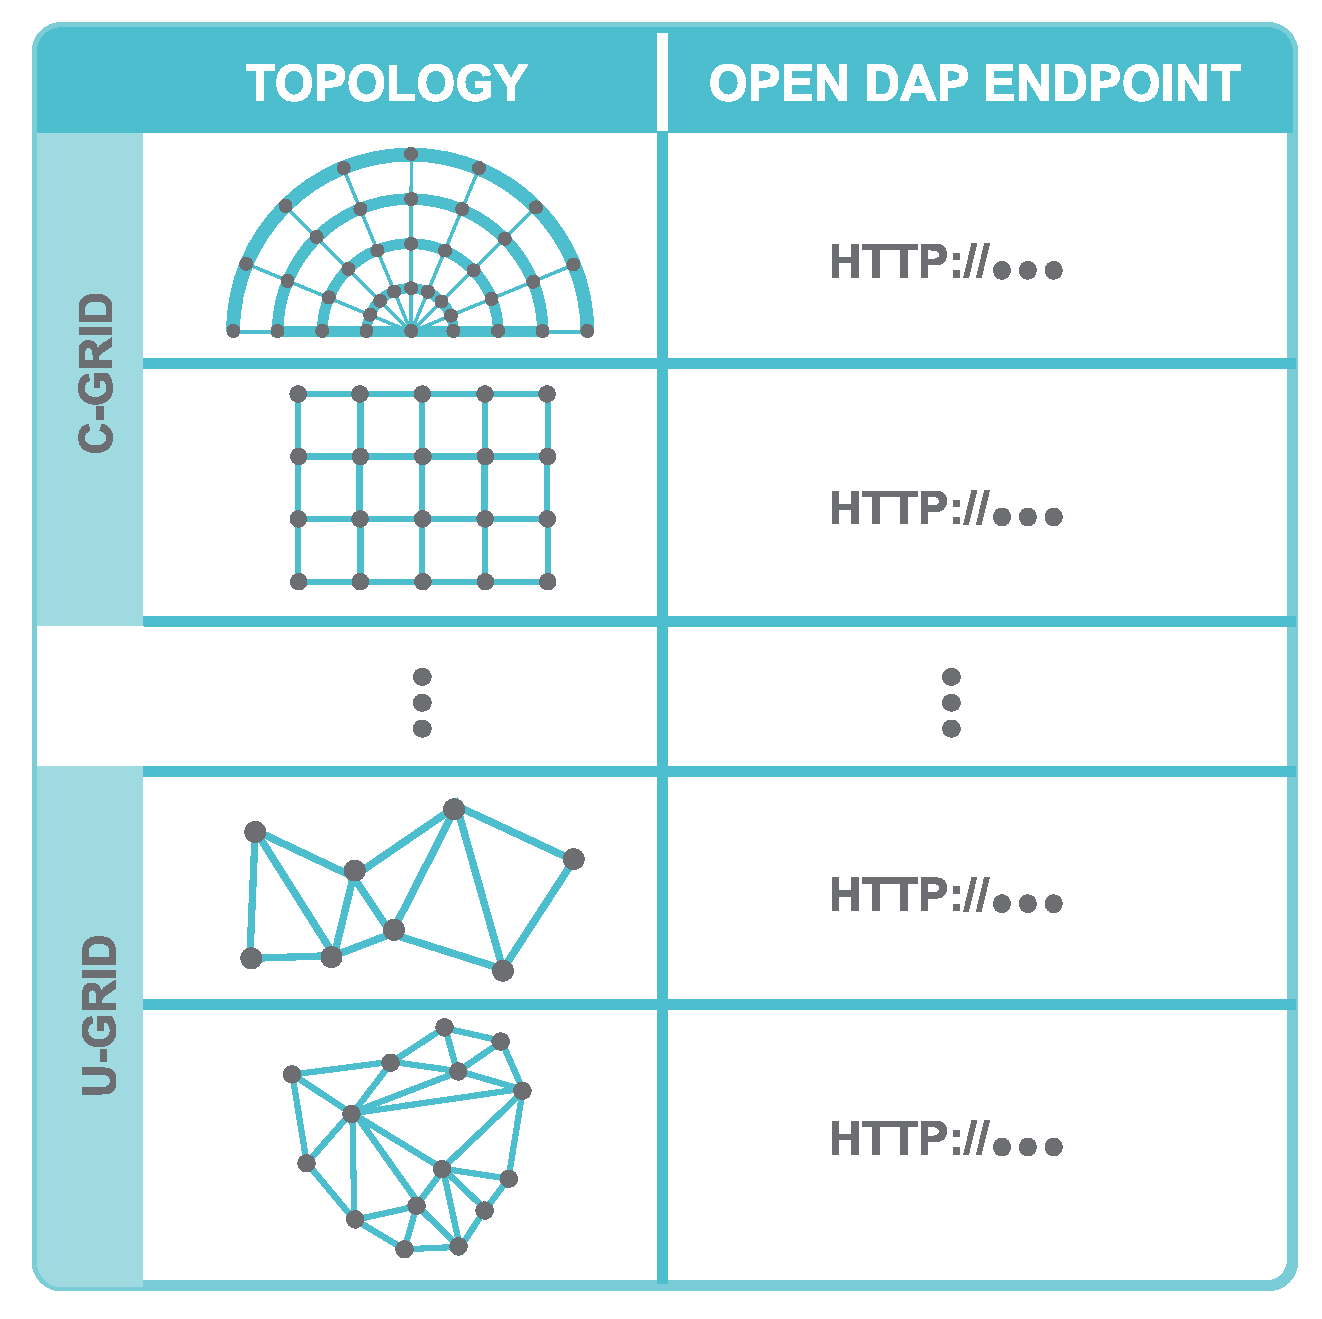
\includegraphics[height=2in]{../figs/sciwms_book_db_topology_endpoint_chart}
%%   \caption{\Sciwms{} topology and endpoint data store.}
%%   \label{fig:sciwms_topology_endpoints}
%% \end{figure}
